
\begin{frame}
  \frametitle{SPICE: Simulation Program with Integrated Circuit Emphasis}
  \begin{columns}
    \begin{column}{.7\textwidth}
      % In few words
      \begin{itemize}
      \item Developed by Dr. Laurence Nagel in 1973 at Berkeley % University of California
      \item \textbf{First software} to combine \\
        DC, AC and transient analog circuit analysis capabilities
      \item An early \textbf{open source} software initiative (Public Domain)
      \item \textbf{Used in undergraduate courses}
      \item \textbf{Evolved to a worldwide standard} % integrated circuit simulator
      \item \textbf{IEEE Milestone} on February 4, 2011
      \item Berkeley released spice3f5 on 1993 % 6
      \item Superseded by commercial and open source forks \\[1em]
      \end{itemize}
      % What it does ?
      % \begin{itemize}
      % \item Netlist language to describe circuit
      % \item Simulator
      % \end{itemize}
      {\tiny%
        \begin{tabbing}
          To go further \=%
          \href{https://www2.eecs.berkeley.edu/Pubs/TechRpts/1975/9602.html}%
          {SPICE2: A Computer Program to Simulate Semiconductor Circuits; Nagel, Laurence W.; 1975} \\
          \> \href{http://www.omega-enterprises.net/The\%20Origins\%20of\%20SPICE.html}{The Origins of SPICE by Nagel}
        \end{tabbing}%
      }
    \end{column}
    \begin{column}{.3\textwidth}
      \begin{center}
        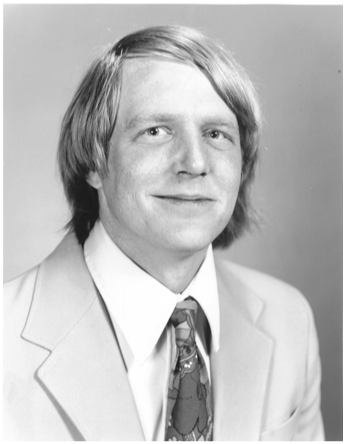
\includegraphics[height=3cm]{images/Larry-Nagel-portrait-young.png} \\[1cm]
        
\includegraphics[width=.7\textwidth]{images/Nagel_Plaque-SCV-2016.png}
      \end{center}
    \end{column}
  \end{columns}
\end{frame}

\begin{frame}[fragile]
  \frametitle{SPICE: Netlist}
  \begin{columns}
    \begin{column}{.5\textwidth}
      \begin{center}
        \includegraphics[width=.9\textwidth]{figures/ac-coupled-amplifier.pdf}
      \end{center}
    \end{column}
    \begin{column}{.5\textwidth}
      \footnotesize
      \begin{Verbatim}[commandchars=\\\{\}]
AC-coupled amplifier
\colorR{V}\colorM{pwr} \colorB{6 0} \colorG{DC 15V}
\colorR{V}\colorM{in} \colorB{1 0} \colorG{AC 1V SIN(0V .5V 1KHz)}
\colorR{C}\colorM{1} \colorB{1 2} \colorG{10u}
\colorR{R}\colorM{1} \colorB{6 2} \colorG{100k}
\colorR{R}\colorM{2} \colorB{2 0} \colorG{20k}
\colorR{R}\colorM{C} \colorB{6 4} \colorG{10k}
\colorR{Q}\colorM{1} \colorB{4 2 3} \colorG{bjt}
\colorR{R}\colorM{E} \colorB{3 0} \colorG{2k}
\colorR{C}\colorM{2} \colorB{4 5} \colorG{10u}
\colorR{R}\colorM{L} \colorB{5 0} \colorG{1Meg}
\colorG{.model bjt npn(bf=80 cjc=5p rb=100)}
\colorO{.ac dec 5 10m 1G}
\colorO{*.tran .02ms 2ms 0 .01ms}
\colorO{.control}
\colorO{run}
\colorO{plot V(1) V(5)}
\colorO{.end}
      \end{Verbatim}
      \normalsize
    \end{column}
  \end{columns}
\end{frame}

\begin{frame}[fragile]
  \frametitle{SPICE: A Worldwide Standard for integrated circuit simulation}
  \centerline{Device manufacturers use SPICE language to provide models as sub-circuit}
  \begin{columns}
    \begin{column}{.5\textwidth}
      \begin{center}
        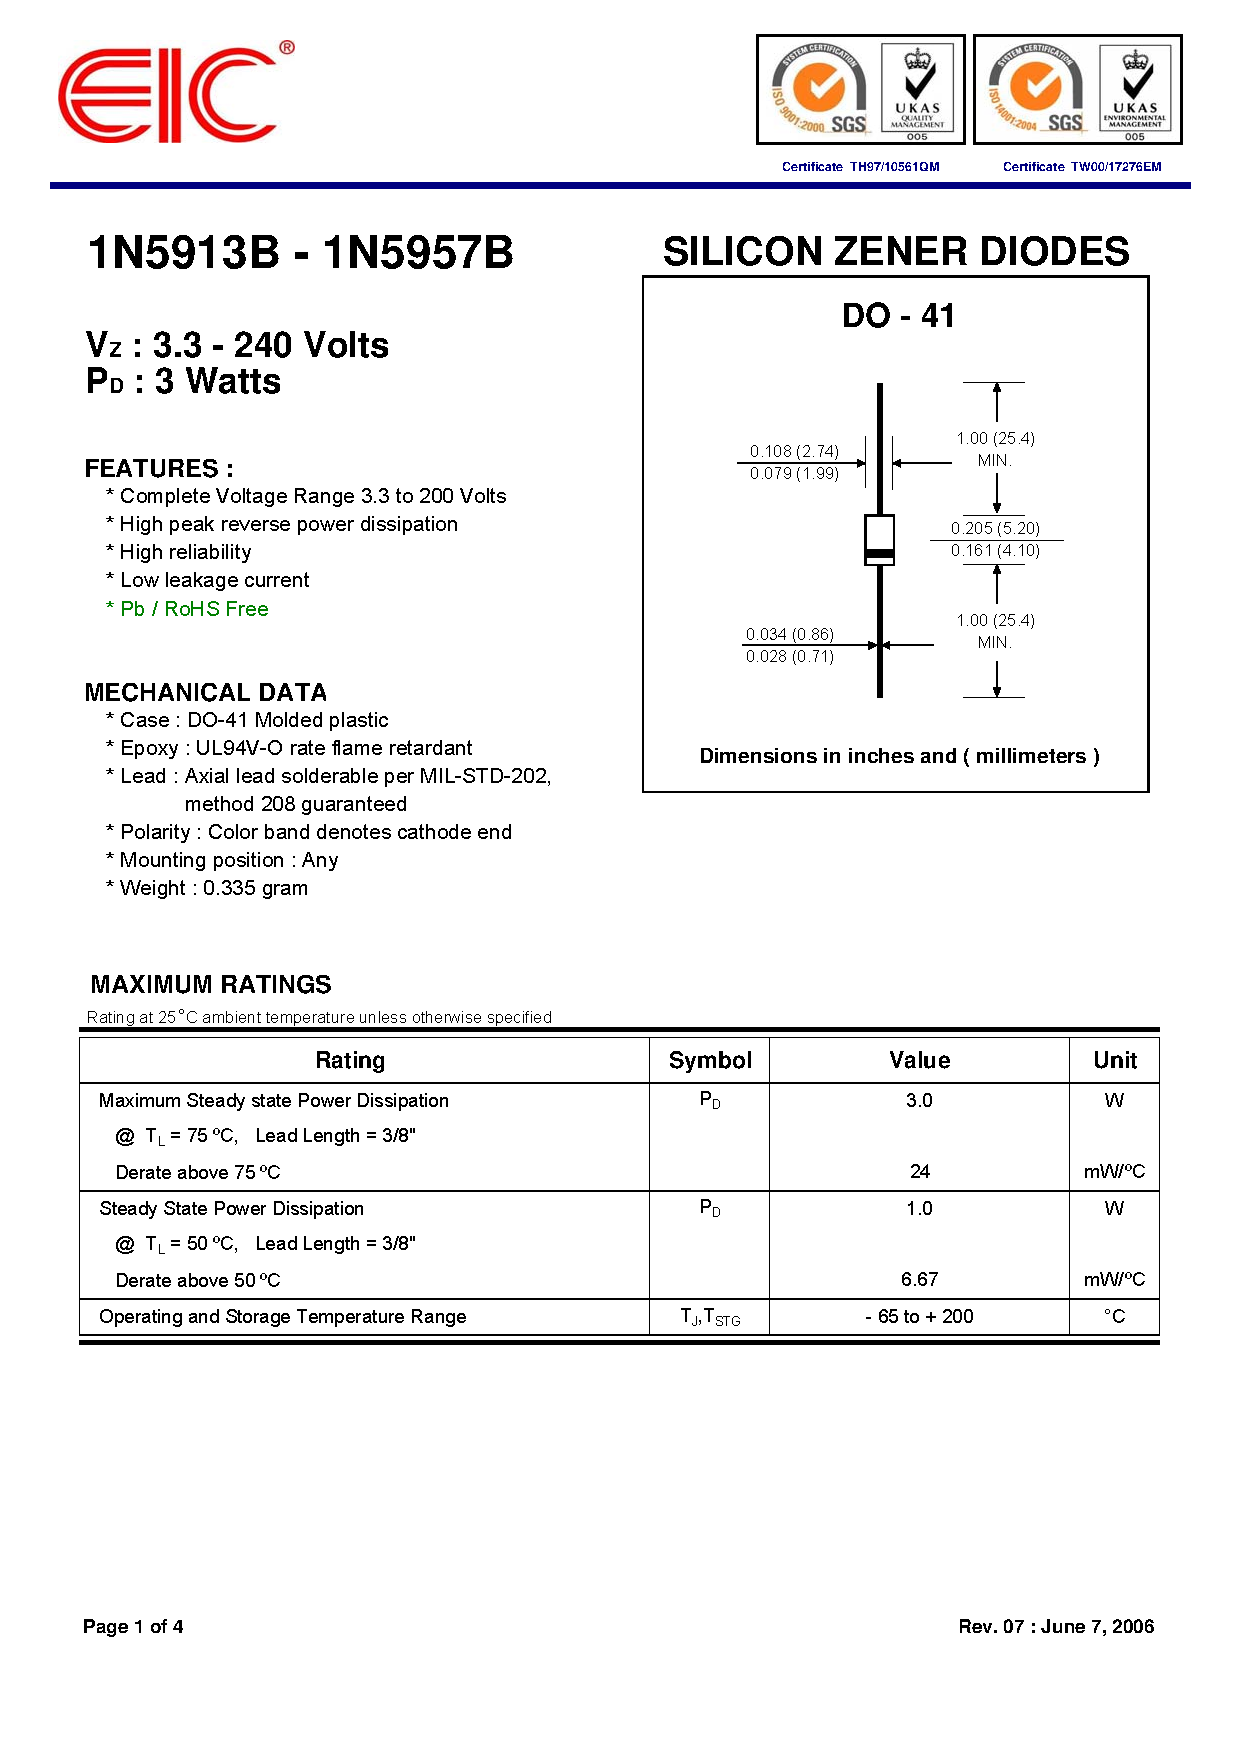
\includegraphics[height=6cm]{figures/1N5919B-1.pdf}
      \end{center}
    \end{column}
    \begin{column}{.5\textwidth}
      \fontsize{4.25pt}{4.25pt}\selectfont
      \begin{Verbatim}[commandchars=\\\{\}]
* http://www.onsemi.com/pub_link/Collateral/1N5919BRL.SP3
\colorR{.SUBCKT d1n5919brl 2 1}
**************************************
*      Model Generated by MODPEX     *
*Copyright(c) Symmetry Design Systems*
*         All Rights Reserved        *
*    UNPUBLISHED LICENSED SOFTWARE   *
*   Contains Proprietary Information *
*      Which is The Property of      *
*     SYMMETRY OR ITS LICENSORS      *
*    Modeling services provided by   *
* Interface Technologies www.i-t.com *
**************************************
* Model generated on Jun 22, 2004
* MODEL FORMAT: SPICE3
\colorO{*     anode cathode}
\colorO{*node: 2      1}
\colorO{*    Forward Section}
\colorB{D1 2 1 MD1}
\colorG{.MODEL MD1 D IS=1.33275e-21 N=1 XTI=1 RS=0.1}
\colorG{+ CJO=1e-11 TT=1e-08}
*    Leakage Current
\colorB{R 1 2 600000 MDR}
\colorG{.MODEL MDR R TC1=0 TC2=0}
*    Breakdown
\colorB{RZ 2 3 0.520393}
\colorB{IZG 4 3 0.3204}
\colorB{R4 4 3 100}
\colorB{D3 3 4 MD3}
\colorG{.MODEL MD3 D IS=2.5e-12 N=2.40102 XTI=0 EG=0.1}
\colorB{D2 5 4 MD2}
\colorG{.MODEL MD2 D IS=2.5e-12 N=3.19856 XTI=0 EG=0.1}
\colorB{EV1 1 5 6 0 1}
\colorB{IBV 0 6 0.001}
\colorB{RBV 6 0 5153.19 MDRBV}
\colorG{.MODEL MDRBV R TC1=1.79e-08}
*-- SPICE3 DIODE MODEL DEFAULT PARAMETER
*  VALUES ARE ASSUMED
*IS=1E-14 RS=0 N=1 TT=0 CJO=0
*VJ=1 M=0.5 EG=1.11 XTI=3 FC=0.5
*KF=0 AF=1 BV=inf IBV=1e-3 TNOM=27
\colorR{.ENDS d1n5919brl}
      \end{Verbatim}
      \normalsize
    \end{column}
  \end{columns}
\end{frame}

%%% Local Variables:
%%% mode: latex
%%% TeX-master: "master"
%%% End:
